

%\documentclass[a4paper]{jarticle}


\section{mdtree.rb Draw decision tree model by PMML \label{sect:mdtree}}
\index{mdtree@mdtree}

The command visualize the decision tree model described in PMML  (Predictive Model Markup Language) and generate a visual diagram in HTML format with D3 library. 
The command is created to visualize the output generated from  \verb|mbonsai| command, and it can be applied to decision tree models in PMML format generated by other software. 

PMML defines description of  values and categories of branch rules, however, it does not record the presence of sequence pattern in  \verb|mbonsai|. 
Therefore, \verb|mbonsai| defines the extension tag to record the branching of sequence pattern, and mdtree.rb allow users to visual the expansion tag of the decision tree.  
  
 The following examples illustrates the series of decision trees constructed with  \verb|mbonsai|. 


\begin{table}[htbp]
\begin{center}
\begin{tabular}{c}

\begin{minipage}{0.5\hsize}
\begin{center}
\caption{Input data dat1.csv. Refer to examples for all data.  \label{tbl:mdtree_input1}}
{\small
\begin{tabular}{crlc}
\hline
Gender&VisitGap&PurchasePattern&Hospitalized \\
\hline
Male&1.2&ABCAAA&Yes\\
Male&10.5&BCDADD&Yes\\
Male&0.5&AAAA&No\\
Male&2.0&BBCC&No\\
Male&3.1&DEDDA&Yes\\
Female&0.7&CCCAA&No\\
Female&1.5&DDDEEE&Yes\\
Female&2.6&BACD&Yes\\
Female&3.5&ABBB&Yes\\
Female&4.0&DDDD&Yes\\
Female&2.1&DEDE&No\\
:&:&:&:\\
\hline
\end{tabular} 
}
\end{center}
\end{minipage}

\end{tabular} 
\end{center}
\end{table} 

Table \ref{tbl:mdtree_input1} shows the training data for the construction of decision tree model with \verb|mbonsai| command. 
The decision tree is saved as PMML file \verb|model.pmml| in the directory specified at \verb|O=|. 
 

\begin{Verbatim}[baselinestretch=0.7,frame=single]
$ mbonsai c=Hospitalized n=VisitGap p=PurchasePattern d=Gender i=dat1.csv O=outdat
#END# kgbonsai O=outdat c=Hospitalized d=Gender i=dat1.csv n=VisitGap p=PurchasePattern; IN=81;
$ ls outdat
alpha_list.csv model.pmml     model.txt      model_info.csv param.csv      predict.csv
\end{Verbatim}

The following command can be used to visualize \verb|model.pmml|. 
The output is rendered as  \verb|model.html| as shown in Figure \ref{fig:mdtree_tree_1}. 



\begin{Verbatim}[baselinestretch=0.7,frame=single]
$ mdtree.rb i=outdat/model.pmml o=model.html
#END# mdtree.rb i=outdat/model.pmml o=model.html;
$ open model.html 
\end{Verbatim}

\begin{figure}[htbp]
\begin{center}
\begin{tabular}{c}

\begin{minipage}{0.9\hsize}
\begin{center}
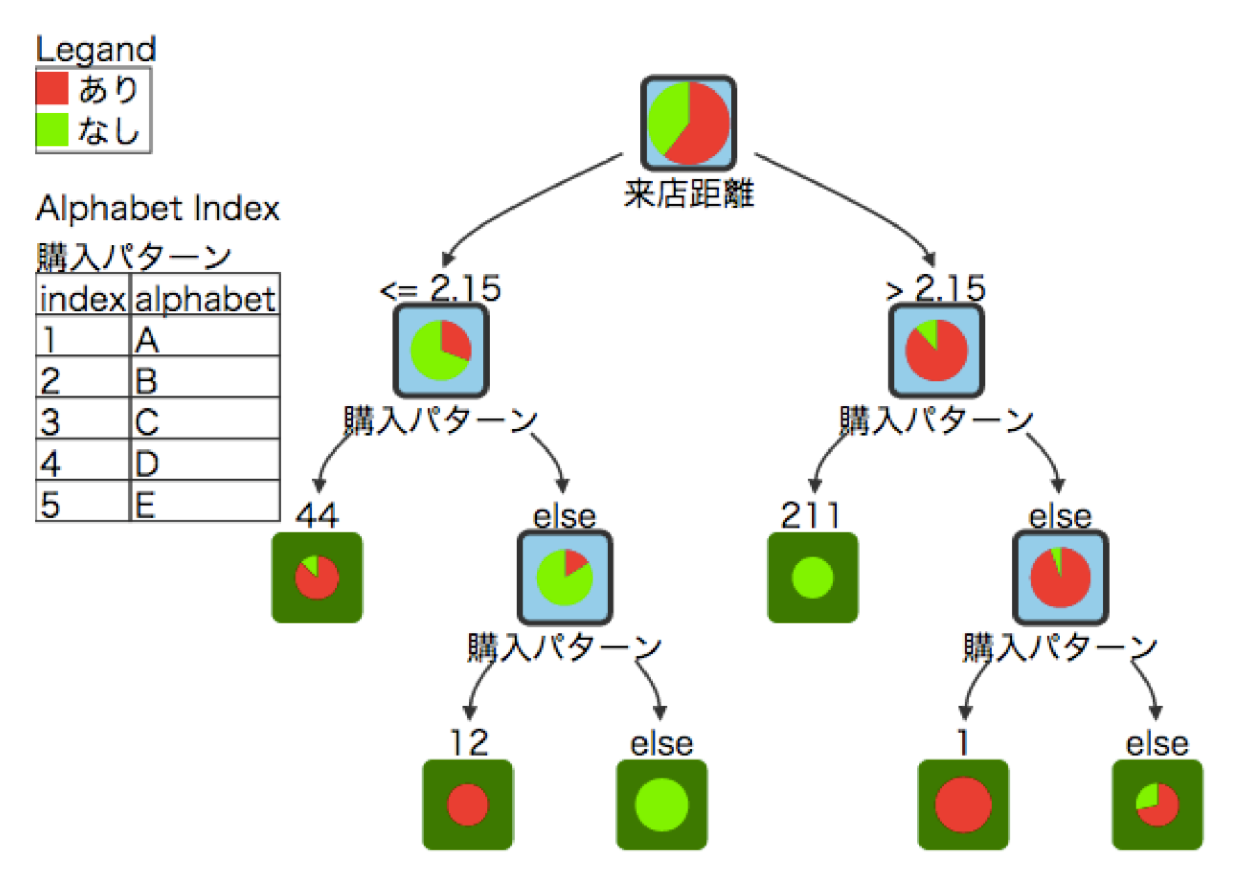
\includegraphics[scale=0.5]{figure/tree_1.eps}
\caption{Draw decision tree with this command.  
The pie chart inside each node shows the class distribution (color for each class is shown in legend). 
The node with dotted line represents an intermediate node, the node with solid line represents a leaf node. 
The item name for the branch is shown below the node, and the branch rule is shown above the node. 
For example, on the first child level, if the Visit gap is below 2.15 on the left, and more than 2.15 on the right branch with no overlaps on both. 
When the node contains a sequence pattern, the branch which contained the pattern will be shown on the left, and the branch without the pattern is shown on the right. 
For instance, the left node in the second level from the top shows the purchase pattern containing ``44". 
 Furthermore, the characters of sequence patterns and each corresponding index are shown in the alphabet-index table in the upper left of the figure.
\label{fig:mdtree_tree_1}}
\end{center}
\end{minipage}

\end{tabular}
\end{center}
\end{figure}

The maximum tree built in \verb|mbonsai| is stored, the level of pruning of the decision tree can be controlled by specifying pruning degree at \verb|alpha=|. 
When an integer value that is greater than 0 is specified at \verb|alpha=|, when the decision tree is large, a lot of branches will be pruned. 
When \verb|alpha=| is not specified and cross validation is not specified for \verb|mbonsai|, \verb|alpha=0.01| is specified. Yet if cross validation is specified, minimum misclassification rate is rendered. 

Figure \ref{fig:mdtree_tree_2}l the pruned decision tree with \verb|alpha=0.1|. 

\begin{Verbatim}[baselinestretch=0.7,frame=single]
$ mdtree.rb alpha=0.1 i=outdat/model.pmml o=model2.html
#END# mdtree.rb alpha=0.1 i=outdat/model.pmml o=model.html;
$ open model2.html 
\end{Verbatim}

\begin{figure}[htbp]
\begin{center}
\begin{tabular}{c}

\begin{minipage}{0.5\hsize}
\begin{center}
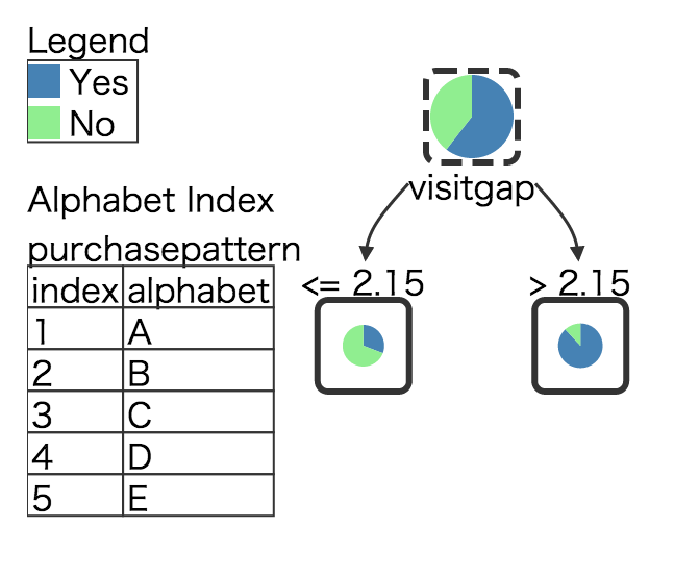
\includegraphics[scale=0.5]{figure/tree_2.eps}
\caption{Decision tree created when pruning degree is set as alpha=0.1\label{fig:mdtree_tree_2}}
\end{center}
\end{minipage}

\end{tabular}
\end{center}
\end{figure}

\subsection{Collaboration with R}

Many decision tree construction packages are available in the R statistical analysis package.
The following section explains how to draw a decision tree with the \verb|rpart| library. 

We will build a decision tree with R script using two data sets - Iris data set (\verb|iris|) and prostate cancer data set (\verb|stagec|).
The decision tree is built using \verb|rpart| libraries and the model saved in PMML output. 

This manual will not go into details on how to build  decision tree model from the content in the data set. Note that PMML, XML, and rpart R libraries must be installed before proceeding with the following examples. 

The program will generate a output from the decision tree of iris and prostate cancer will be saved as PMML file \verb|model_r1.pmml| and \verb|model_r1.pmm2|. 


\begin{Verbatim}[baselinestretch=0.7,frame=single]
library(pmml)
library(rpart)
iris.rp=rpart(Species~.,data=iris)
sink("model_r1.pmml")
pmml(iris.rp)
sink()

stagec$progstat <- factor(stagec$pgstat, levels = 0:1, labels = c("No", "Prog"))
cfit <- rpart(progstat ~ age + eet + g2 + grade + gleason + ploidy, data = stagec, method = "class")
sink("model_r2.pmml")
pmml(cfit)
sink()
\end{Verbatim}

After obtaining two PMML files, we will follow the procedure for drawing a decision tree.
The decision trees are shown in diagrams \ref{fig:mdtree_tree_3} and  \ref{fig:mdtree_tree_3}.  

\begin{Verbatim}[baselinestretch=0.7,frame=single]
$ mdtree.rb i=model_r1.pmml o=out_r1.html
#END# mdtree.rb i=model_r1.pmml o=outl_r1.html;
$ mdtree.rb i=model_r2.pmml o=/out_r2.html
#END# mdtree.rb i=model_r2.pmml o=out_r2.html;
$ open model1_r1.html
$ open model1_r2.html
\end{Verbatim}

\begin{figure}[htbp]
\begin{center}
\begin{tabular}{c}

\begin{minipage}{0.5\hsize}
\begin{center}
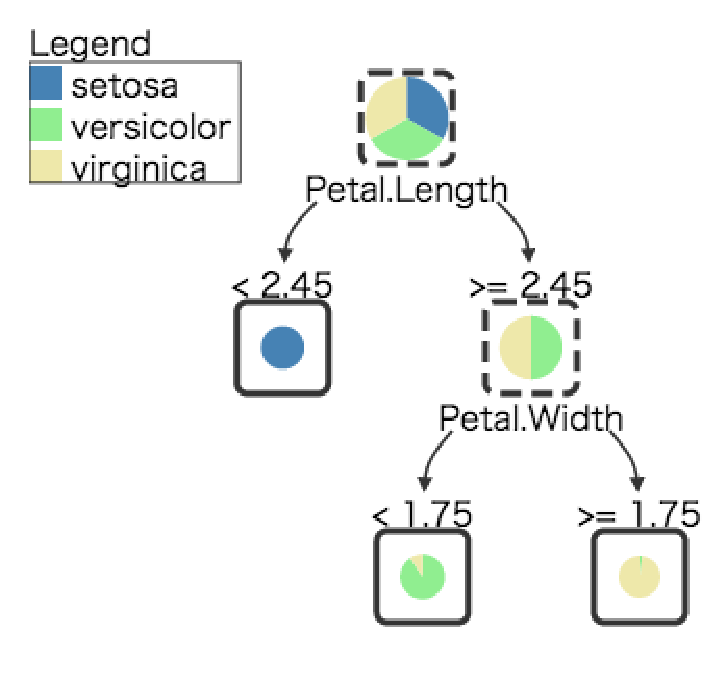
\includegraphics[scale=0.5]{figure/tree_3.eps}
\caption{Decision tree of Iris dataset\label{fig:mdtree_tree_3}}
\end{center}
\end{minipage}

\end{tabular}
\end{center}
\end{figure}

\begin{figure}[htbp]
\begin{center}
\begin{tabular}{c}

\begin{minipage}{0.5\hsize}
\begin{center}
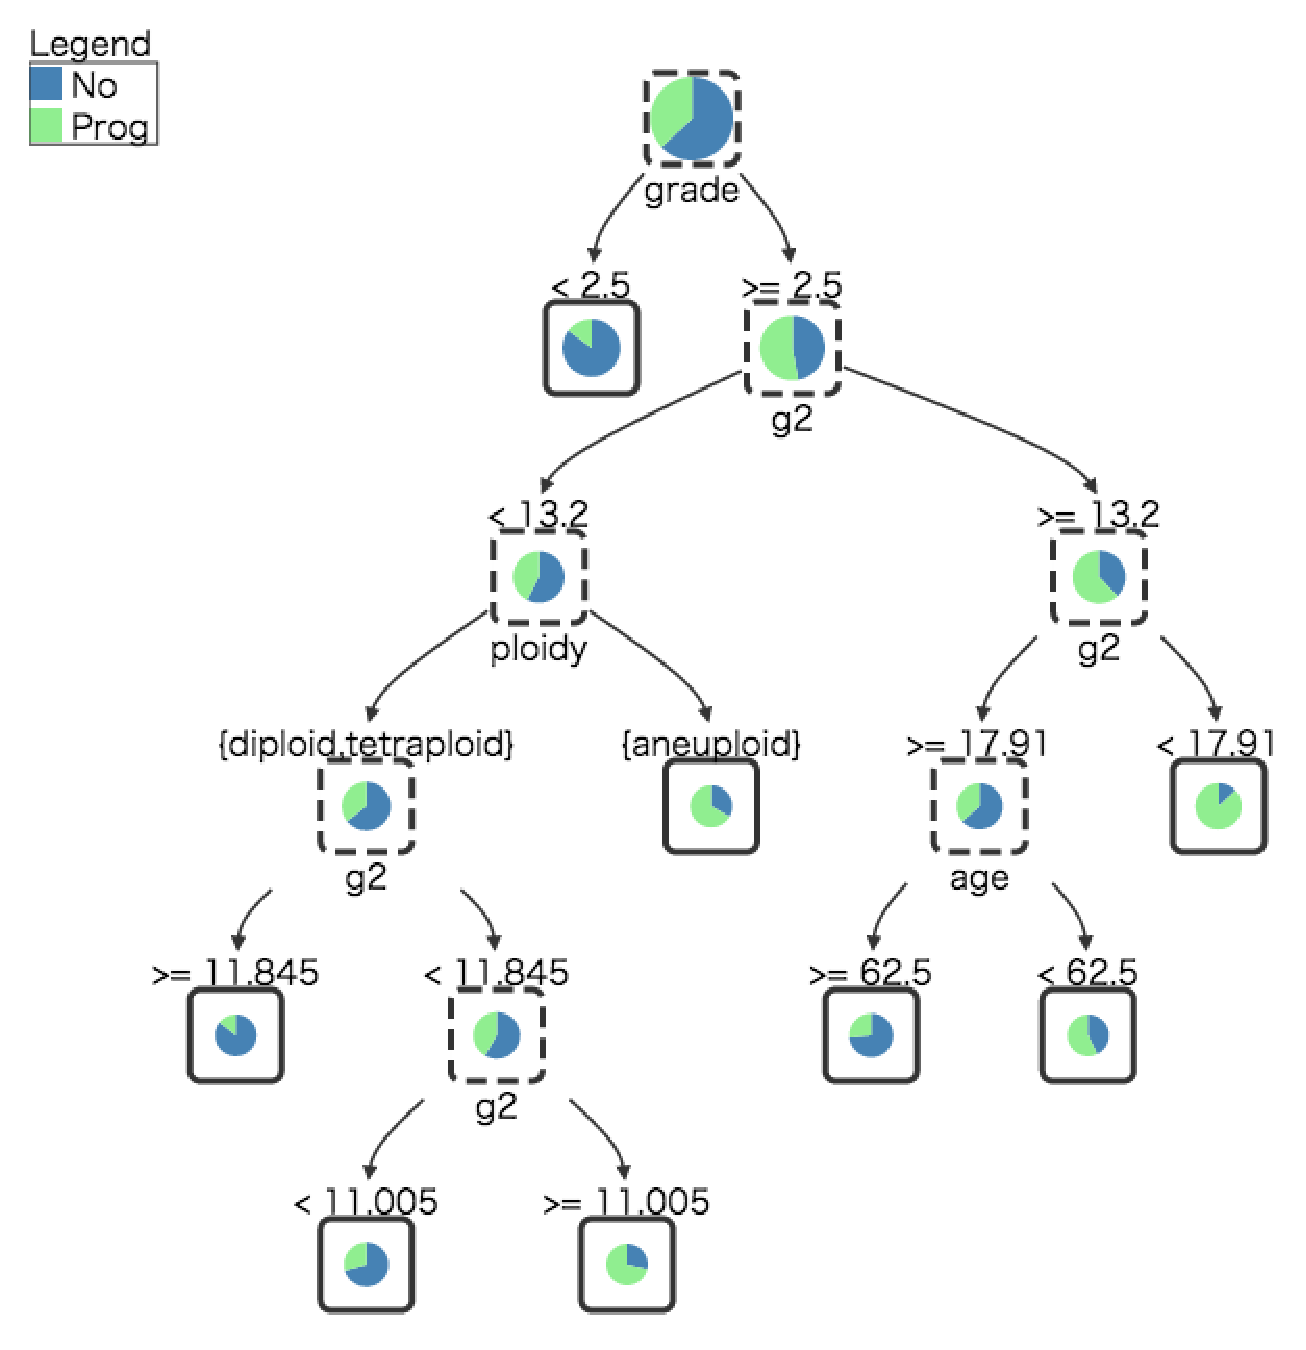
\includegraphics[scale=0.5]{figure/tree_4.eps}
\caption{Decision tree of prostate cancer\label{fig:mdtree_tree_4}}
\end{center}
\end{minipage}

\end{tabular}
\end{center}
\end{figure}



\subsection{Format}
\begin{verbatim}
mdtree.rb i= o= [alpha=] [--help]
\end{verbatim}

\begin{table}[htbp]
{\small
\begin{tabular}{ll}
\verb|i=| & : PMML file of decision tree model \\
\verb|o=| & : Output file (HTML file) \\
\verb|alpha=| & : Specify the pruning degree (more branches are pruned when pruning degree is a integer greater than 0).  \\
              & : when this is not specified,  and cross validation is not specified for \verb|mbonsai|, \\
              & : the value will be set as 0.01. If cross validation is specified, model with the minimum misclassification rate is rendered. \\
              & : This parameter is only valid for building decision trees with \verb|mbonsai|.\\
\verb|--help| & : Show help  \\
\end{tabular} 
}
\end{table} 

\subsection{Example}
\subsubsection*{例1: Basic Example}

Example from the above section.


\begin{Verbatim}[baselinestretch=0.7,frame=single]
$ cat dat1.csv
gender,visitgap,purchasepattern,hospitalized
Male,1.2,ABCAAA,Yes
Male,10.5,BCDADD,Yes
Male,0.5,AAAA,No
Male,2.0,BBCC,No
Male,3.1,DEDDA,Yes
Female,0.7,CCCAA,No
Female,1.5,DDDEEE,Yes
Female,2.6,BACD,Yes
Female,3.5,ABBB,Yes
Female,4.0,DDDD,Yes
Female,2.1,DEDE,No
Male,1.2,ABCAAA,Yes
Male,10.5,BCDADD,Yes
Male,0.5,AAAA,No
Male,2.0,BBCC,No
Male,3.1,DEDDA,Yes
Male,0.7,CCCAA,No
Male,1.5,DDDEEE,No
Male,2.6,BACD,Yes
Male,3.5,ABBB,Yes
Male,4.0,DDDD,Yes
Male,2.1,DEDE,No
Male,1.2,ABCAAA,Yes
Male,10.5,BCDADDA,Yes
Male,0.5,AAAAA,No
Male,2.0,BBCCA,No
Male,3.1,DEDDA,Yes
Male,0.7,CCCAA,No
Male,1.5,ADDDEEE,Yes
Male,2.6,BACD,Yes
Male,3.5,ABBB,Yes
Male,4.0,DDDD,Yes
Female,2.1,DEDE,No
Female,1.2,ABCAAA,Yes
Female,10.5,BCDADD,Yes
Female,0.5,AAAA,No
Female,2.0,BBCC,No
Female,3.1,DEDDA,Yes
Female,0.7,CCCAA,No
Female,1.5,DDDEEE,Yes
Female,2.6,BACD,Yes
Female,3.5,ABBB,Yes
Female,4.0,DDDD,Yes
Female,2.1,DEDE,No
Female,1.2,ABCAAA,Yes
Female,10.5,BCDADD,Yes
Female,0.5,AAAA,No
Female,2.0,BBCC,No
Female,3.1,DEDDA,Yes
Female,0.7,CCCAA,No
Female,1.5,DDDEEE,Yes
Female,2.6,BACD,Yes
Female,3.5,ABBB,Yes
Female,1.0,DDDD,Yes
Female,2.5,DEDE,No
Female,2.5,ABBB,Yes
Female,1.0,DDDD,Yes
Female,1.1,DEDE,No
Female,2.2,ABCAAA,Yes
Female,10.5,BCDADD,Yes
Female,1.5,AAAA,No
Female,2.6,BBCC,No
Female,3.3,DEDDA,Yes
Female,1.7,CCCAA,No
Female,1.5,DDDEEE,Yes
Female,2.6,BACD,Yes
Female,3.9,ABBB,Yes
Female,4.5,DDDD,Yes
Female,2.1,DEDE,No
Female,3.9,BABB,Yes
Male,4.5,BAA,No
Female,2.1,DEDE,No
Male,3.9,BABB,Yes
Female,3.9,BABB,Yes
Male,4.5,BAA,No
Female,2.1,DEDE,No
Male,3.9,BABB,Yes
Female,3.9,BABB,Yes
Male,4.5,BAA,No
Female,2.1,DEDE,No
Male,3.9,BABB,Yes
$ mbonsai c=hospitalized n=visitgap p=purchasepattern d=gender i=dat1.csv O=outdat
ABCDE = 12345  *improved(errev:0.037037 *improved(errMin:0,leaf:1)
#END# kgbonsai O=outdat c=hospitalized d=gender i=dat1.csv n=visitgap p=purchasepattern
N=81
$ mdtree.rb i=outdat/model.pmml o=model1.html
#END# /usr/bin/mdtree.rb i=outdat/model.pmml o=model1.html
$ mdtree.rb alpha=0.1 i=outdat/model.pmml o=model2.html
#END# /usr/bin/mdtree.rb alpha=0.1 i=outdat/model.pmml o=model2.html
$ head model1.html
<html lang="ja">
<head>
  <meta charset="utf-8">
	<meta name="viewport" content="width=device-width, initial-scale=1.0">
  <style type="text/css">
	  p.title { border-bottom: 1px solid gray
		g > .type-node > rect { stroke-dasharray: 10,5
hite
		g > .type-leaf > rect { stroke-width: 3px
		.edge path {  fill: none
		svg >.legend > rect { stroke-width: 1px
$ head model2.html
<html lang="ja">
<head>
  <meta charset="utf-8">
	<meta name="viewport" content="width=device-width, initial-scale=1.0">
  <style type="text/css">
	  p.title { border-bottom: 1px solid gray
		g > .type-node > rect { stroke-dasharray: 10,5
hite
		g > .type-leaf > rect { stroke-width: 3px
		.edge path {  fill: none
		svg >.legend > rect { stroke-width: 1px
\end{Verbatim}


%\end{document}

